\documentclass{article}
\usepackage[margin=1in]{geometry}
\usepackage{amsmath,amsthm,amssymb}
\usepackage{bbm,enumerate,mathtools}
\usepackage{tikz,pgfplots}
\usepackage{chessboard}
\usepackage[hidelinks]{hyperref}
\usepackage{multicol} % Problem 35

\newenvironment{question}{\begin{trivlist}\item[\textbf{Question.}]}{\end{trivlist}}
\newenvironment{note}{\begin{trivlist}\item[\textbf{Note.}]}{\end{trivlist}}
\newenvironment{references}{\begin{trivlist}\item[\textbf{References.}]}{\end{trivlist}}
\newenvironment{related}{\begin{trivlist}\item[\textbf{Related.}]\end{trivlist}\begin{enumerate}}{\end{enumerate}}


\begin{document}
  Consider all rectangles composed of $n$ squares such that the greatest common
  divisor of all the sidelengths is 1.

\begin{figure}[!h]
  \centering
  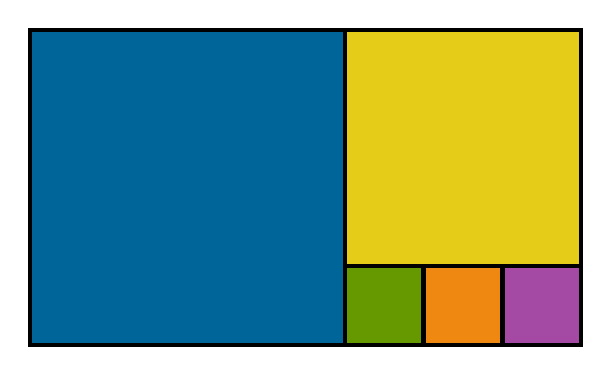
\begin{tikzpicture}
    \draw[ultra thick, fill={rgb:red,0;green,2;blue,3}] (0,0) rectangle (4,4);
    \draw[ultra thick, fill={rgb:red,1;yellow,8;blue,1}] (4,1) rectangle (7,4);
    \draw[ultra thick, fill={rgb:red,2;green,3;blue,0}] (4,0) rectangle (5,1);
    \draw[ultra thick, fill={rgb:red,6;yellow,8;blue,1}] (5,0) rectangle (6,1);
    \draw[ultra thick, fill={rgb:red,5;blue,5;white,4}] (6,0) rectangle (7,1);
  \end{tikzpicture}\hspace{1cm}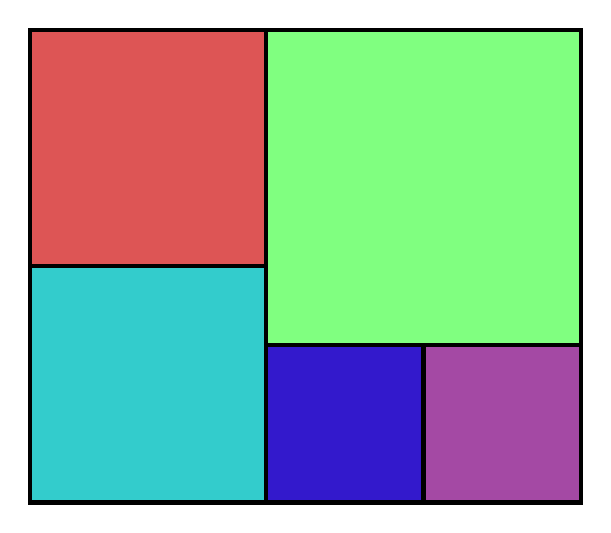
\begin{tikzpicture}
      \draw[ultra thick, fill={rgb:red,2;cyan,8}] (0,0) rectangle (3,3);
      \draw[ultra thick, fill={rgb:red,8;yellow,2;blue,2;white,3}] (0,3) rectangle (3,6);
      \draw[ultra thick, fill={rgb:red,0.5;yellow,0.5;blue,4}] (3,0) rectangle (5,2);
      \draw[ultra thick, fill={rgb:red,5;blue,5;white,4}] (5,0) rectangle (7,2);
      \draw[ultra thick, fill={rgb:green,5;white,5}] (3,2) rectangle (7,6);
    \end{tikzpicture}
  \caption{
    Two examples of rectangles made from $n=5$ squares.
    In the first $\gcd(1, 1, 1, 3, 4) = 1$ and in the second
    $\gcd(2,2,3,3,4) = 1$.
  }
\end{figure}

\begin{question}
  Given $n$ squares, how many such rectangles exist?
\end{question}
\begin{related}
  \item How many ways are there to make convex polygons out of $n$ equilateral triangles?
  \item How many ways are there to make cuboids out of $n$ cubes?
\end{related}
\end{document}
